%Autor: Aarón Martín Castillo Medina.
%Asesora: Dra. Katya Rodríguez Vázquez
%Contacto: katya.rodriguez@iimas.unam.mx; amcm329@hotmail.com

%El siguiente archivo contempla los fundamentos que dan origen 
%a los M.O.E.A.'s, los cuales son: Algoritmos Evolutivos y 
%Optimización Multiobjetivo.


%Se indica que el documento es de tipo reporte bajo el paquete standalone.
\documentclass[class=report, crop=false]{standalone}

%Se cargan todos los paquetes que residen en el archivo packages_used_standard.sty
\usepackage{packages_used_standard}

%Comienza el documento.
\begin{document}

%Inicia el desarrollo del Capítulo relacionado con los 
%fundamentos en los que está basado el M.O.E.A.
\chapter{Fundamentos}
Para comprender la composición y funcionamiento de un M.O.E.A. 
\textbf{(Multi-Objective Evolutionary Algorithm ó Algoritmo 
Evolutivo Multiobjetivo)} es necesario adentrarse en sus raíces, 
más en específico éste tiene sus fundamentos principalmente en 
las siguientes disciplinas:

\begin{itemize}
\item Algoritmos Evolutivos
\item Optimización Multiobjetivo
\end{itemize}

Cada uno de manera individual comprende por sí mismo una colección 
magna de conocimiento, por lo que se explicarán de manera breve pero 
precisa enfocando los detalles de tal manera que lo que se describa 
en este capítulo empate con la generalización del M.O.E.A. en el 
siguiente episodio.\break
A continuación se muestran cada uno estos tópicos:

%Inicia la sección destinada a tratar de manera somera a los
%Aloritmos Evolutivos, haciendo énfasis en su procedimiento y 
%técnicas auxiliares.
\section{Algoritmos Evolutivos}
Se denominan Algoritmos Evolutivos al conjunto de heurísticas 
\footnote{Aproximación de una solución donde es difícil o imposible 
hallar una idónea bajo las condiciones y métodos originales.} 
basadas en procesos progresivos tales como las teorías de Darwin 
relativas la selección natural \footnote{Concepto que corresponde 
a una colaboración con Alfred Wallace previo al trabajo de Darwin.} 
y la supervivencia del individuo más apto \footnote{Término acuñado 
por Herber Spencer posterior a la publicación de la obra de Darwin.}, 
de hecho citándolo en su \textit{magnum opus} \cite{b1} se puede 
tomar la siguiente frase que engloba todo el procedimiento:\medskip\break
\textit{``Es interesante contemplar un enmarañado ribazo cubierto 
por muchas plantas de varias clases, con aves que cantan en los 
matorrales, con diferentes insectos que revolotean y con gusanos 
que se arrastran entre la tierra húmeda, y reflexionar que estas 
formas, primorosamente construidas, tan diferentes entre sí y que 
dependen mutuamente de modos tan complejos, han sido producidas 
por leyes que obran a nuestro alrededor.\medskip\break
Estas leyes, tomadas en un sentido más amplio, son: la de crecimiento 
con reproducción; la de herencia, que casi está comprendida en la 
de reproducción; la de variación por la acción directa e indirecta 
de las condiciones de vida y por el uso y desuso; una razón del 
aumento, tan elevada, tan grande, que conduce a una lucha por la 
vida, y como consecuencia a la selección natural, que determina 
la divergencia de caracteres y la extinción de las formas menos 
perfeccionadas''}.\medskip\break
De esta manera los Algoritmos Evolutivos toman estos conceptos y 
los trasladan a un entorno cuantificable y tecnológico; así el 
objetivo reside entonces en encontrar la solución ``óptima'' \textbf{(aquélla 
que sea ideal o la que se le aproxime mejor)} ante una problemática 
establecida, esto a través de mecanismos de selección y recombinación 
que permitan un adecuado refinamiento y por tanto la obtención 
de respuestas cada vez más cercanas a las requeridas.\medskip
\begin{figure}[ht]
%Se coloca el vínculo interno procedente del capítulo 2 (c2_1).
\label{sec:c2_1}
\centering
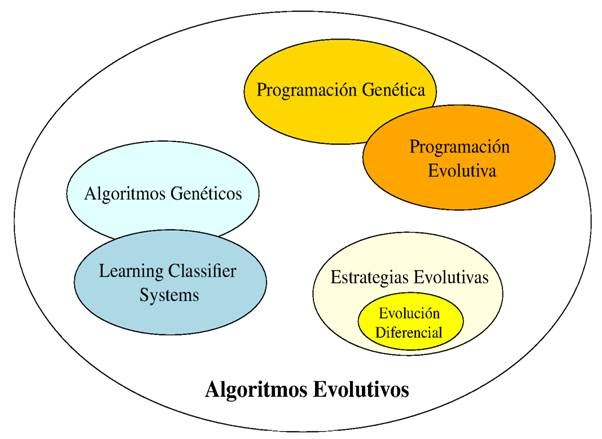
\includegraphics[width=12.8cm,height=8.1cm]{c21.jpg}
\caption{Esbozo gráfico de las distintas ramificaciones de los Algoritmos Evolutivos}
\end{figure}\break
Abordando un poco de contexto histórico éstas surgen en la década 
de 1950, sin embargo tuvieron su momento álgido hasta 1960 debido 
en gran medida a la creación de computadoras cada vez más potentes 
ya que como el lector podrá notar en secciones posteriores los 
recursos para llevar a cabo la ejecución de estos algoritmos no 
son pocos; por otra parte la concepción de dicho género pertenece 
a una rama más general denominada Cómputo Evolutivo en la cual 
han intervenido varios científicos para su forjamiento, sólo por 
mencionar algunos se tiene a Lawrence Jerome Fogel, John Henry 
Holland e Ingo Rechenberg, los cuales son los creadores de la 
Programación Evolutiva, Algoritmos Genéticos y las Estrategias 
Evolutivas respectivamente.\medskip\break
Cabe mencionar que la diferencia entre todas estas subdisciplinas 
radica en el hecho de que el proceso evolutivo aunque es esclarecedor 
también es genérico, motivo por el cual existen tantas ramificaciones 
de los Algoritmos Evolutivos como versiones de dicho procedimiento 
biológico y por ende de obtención de resultados.\medskip\break
Para fines del proyecto se considerarán únicamente a los Algoritmos 
Genéticos y las Estrategias Evolutivas debido a su implementación 
sencilla y abundancia de ejemplos, no obstante para proporcionar 
al lector de un panorama más amplio se muestra en la \hyperref[sec:c2_1]{\textcolor{blue}{Figura 2.1}} 
el diagrama con la mayoría de las técnicas que conforman a los 
Algoritmos Evolutivos.\medskip\break
Aún considerando el aspecto global del proceso evolutivo es 
posible precisar las etapas que determinan su comportamiento, 
de esta manera se toma una convención sobre las características 
mínimas que debe tener en cuenta una implementación en este 
rubro.\break
Tomando como base la \hyperref[sec:c2_2]{\textcolor{blue}{Figura 2.2}} 
se le presentan al lector no sólo las fases del procedimiento, 
sino también el orden en el que se llevan a cabo. A continuación 
se realiza una breve descripción:\medskip
\begin{figure}[ht]
%Se coloca el vínculo interno procedente del capítulo 2 (c2_2).
\label{sec:c2_2}
\centering
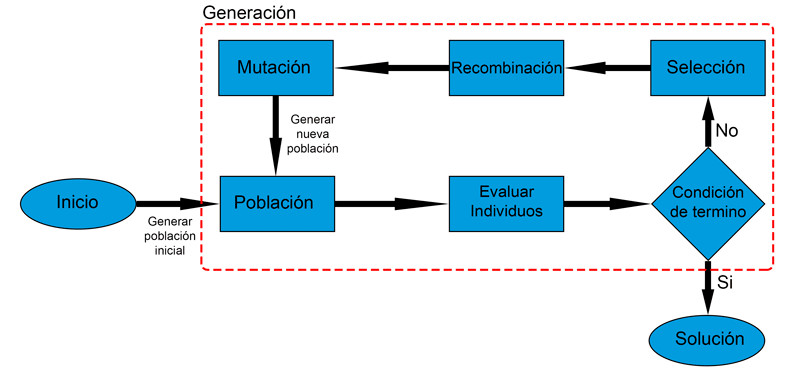
\includegraphics[width=13.5cm,height=7.9cm]{c22.png}
\caption{Fases del proceso evolutivo}
\end{figure}\break
En \textbf{Inicio} y \textbf{Población} la computadora ofrece 
un conjunto inicial de elementos aleatorios conocidos como 
\textit{individuos}, los cuales son los candidatos a la solución 
óptima, lo anterior indica que, debido a la naturaleza de su 
creación, existirán inicialmente individuos que no se acerquen 
tanto a la meta ideal como otros.\break
Como dato adicional, en algunas fuentes **(poner fuentes)** se 
utiliza el término \textit{cromosomas} para referirse de igual 
manera a dicho conjunto, sin embargo en este proyecto ambas 
palabras tendrán acepciones distintas.\medskip\break
La parte \textbf{Evaluar Individuos} implica la asignación de 
un valor escalar que determine la calidad de un individuo frente 
al problema que debe resolver. Para esto se apoya de un factor 
conocido como \hyperref[sec:c2_3]{\textbf{\textcolor{blue}{aptitud}}}.\medskip\break
La idea es entonces evolucionar a los individuos a través de 
técnicas que emulen la selección natural \hyperref[sec:c2_4]{\textbf{\textcolor{blue}{(Selección)}}}
y la generación de nuevos elementos \hyperref[sec:c2_5]{\textbf{\textcolor{blue}{(Recombinación ó Cruza}}}, \hyperref[sec:c2_6]{\textbf{\textcolor{blue}{Mutación)}}}) con la finalidad de obtener descendientes cada vez 
más aptos que, como se mencionó al principio, se acerquen más 
a la solución idónea.\break
Al proceso de creación de un nuevo conjunto de individuos se le 
conoce como \textit{generación}.\medskip\break 
Finalmente en el diagrama la porción correspondiente a \textbf{Condición de Término}
es meramente un requisito que indica que se ha alcanzado un 
límite para evitar que el proceso ecolutivo cicle indefinidamente, 
éste puede ser tanto un número límite de generaciones como un 
requisito alusivo a la aptitud.\medskip\break
Ahora utilizando la \hyperref[sec:c2_7]{\textcolor{blue}{Figura 2.3}} 
se expone de manera más sucinta la estructura interna de un 
individuo, así como algunos factores que giran en torno a 
éste:%\break
\begin{figure}[ht]
\centering
%Se coloca el vínculo interno procedente del capítulo 2 (c2_7).
\label{sec:c2_7}
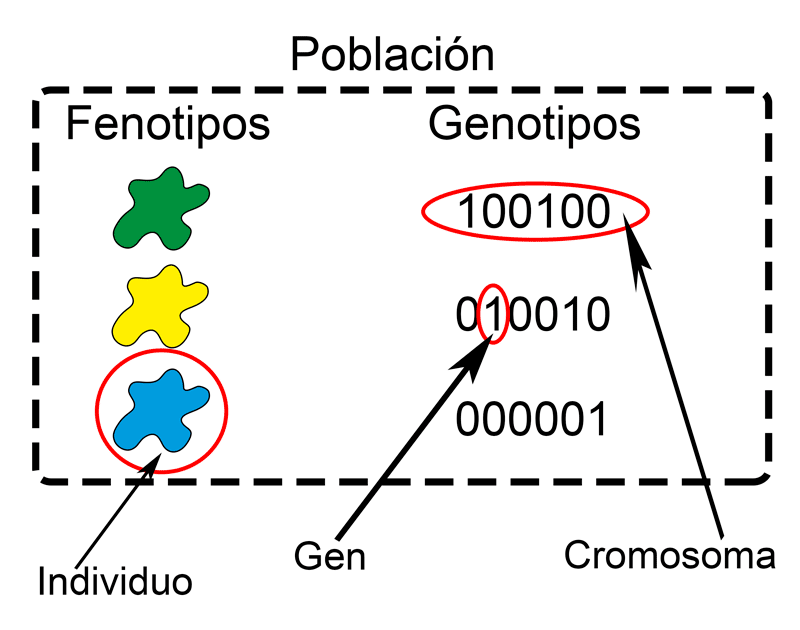
\includegraphics[width=13cm,height=8.1cm]{c23.png}
\caption{Elementos que conforman a un individuo}
\end{figure}\break
El primer término que el lector debe tomar en cuenta es el 
de \textit{población}; éste no es otra cosa que el conjunto 
de dos o más individuos.\break
Un concepto que no aparece aquí pero que será muy utilizado 
tanto en el el producto de software como en el Manual Técnico 
es el de \textit{comunidad}. De acuerdo a las bases biológicas 
\cite{b3} una comunidad es el conjunto de dos o más poblaciones 
y debido a la necesidad de operar con múltiples poblaciones 
simultáneamente en cada uno de los algoritmos se decidió crear 
una entidad con este nombre que no sólo satisfaciera las necesidades 
técnicas sino también que proporcionara un sentido biológico 
inherente al proyecto.\break
Como se aclaró previamente, se decidió mantener una escición
entre los conceptos \textit{cromosoma} e \textit{individuo} 
ya queen secciones posteriores será de gran utilidad puesto que, 
si bien en la práctica ambos conceptos se manejan indistintamente, 
esto ayudará a comprender mejor tanto el proceso evolutivo como 
sus implementaciones.\medskip\break
Entonces se define el cromosoma como una estructura que está 
conformada por elementos varios; tomando en cuenta que en el 
argot biológico ésta contiene proteínas, en el entorno computacional 
contendrá símbolos. Las definiciones que siguen corresponden 
a gen y alelo donde básicamente el primero es el espacio donde 
se puede almacenar los elementos antes mencionados respectivamente 
y a su vez el alelo es elemento en sí que va alojado en un gen.\medskip\break  
De lo anterior se incluyen dos conceptos clave que serán de utilidad 
genotipo y fenotipo: mientras que el genotipo se define prácticamente 
como una conjunción de genes (el cromosoma), el fenotipo es considerado 
como el resultado de haber procesado (expresado) el genotipo bajo un 
determinado entorno.

Luego, retomando el nivel de organización mayor conviene 
mencionar además algunos conceptos que van ligados a las 
interacciones entre las comunidades, entre los cuales se encuentran:

\begin{itemize}
\item Presión Selectiva - consiste en la implantación de algún 
tipo de catalizador en una población con la finalidad de obtener al 
mejor individuo generalmente bajo un número pequeño de generaciones. 
\item Especiación - se trata de un proceso en el cual, a partir de 
una población original se deriva al menos un descendiente, los cuales 
puedencompartir apenas pocas características en común. 
\item Epístasis - es considerada una situación en la interacción 
genética (genotipo) en la cual ***(poner referencia)*** una expresión 
de un gen (fenotipo) puede ser modificada radicalmente por la acción 
de dos o más de éstos. En términos más coloquiales la combinación de 
al menos dos genes puede dar un resultado totalmente diferente para 
el que se estaba pensado inicialmente. 
\end{itemize}

Una vez explicado todo el ámbito biológico sobre el cual se va a 
estar laborando, es momento de aterrizar todos estos conceptos 
y relaciones en una perspectiva computacional, se comienza entonces 
por describir de manera más sucinta todo lo relacionado con el 
cromosoma:

%Se inicia esta subsección dando paso a las funciones relacionadas
%con la representación cromosómica.
\subsection{Representación Cromosómica}
%Se coloca el vínculo interno procedente del capítulo 2 (c2_5).
\label{sec:c2_5}
Se define representación cromosómica a la forma de determinar 
el cromosoma y sus propiedades; como ya se mencionó previamente 
el cromosoma será portado por los individuos.\break
Aterrizando lo anterior en un entorno computacional el cromosoma 
consiste en una estructura de almacenamiento tipo arreglo donde cada 
uno de los espacios disponibles (genes) contendrán símbolos (alelos).
Para fines prácticos la representación tiene su base en dos variantes: 
binaria y punto flotante*** poner referencia
La primera sólo puede almacenar valores 1 y 0 en sus alelos mientras 
que la segunda puede almacenar cualquier valor que permita el equipo 
de cómputo en el que se esté implementando.

Una vez erigida la estructura computacional de un cromosoma y de
acuerdo al proceso evolutivo y como un paso intermedio, se debe
obtener el fenotipo, es decir, los resultados de haber procesado el 
genotipo, para ello se debe tomar la función de evaluación descrita al
comienzo y justamente a este paso previo se le denomina "evaluación de la
función objetivo.\break

Dicho lo anterior y con base en las evaluaciones de la función objetivo 
es necesario indicar una métrica que nos permita segmentar a los individuos 
del "peor" al "mejor", a ésta se le conoce como aptitud.

%A continuación se manejan en esta subsección las técnicas manejadas
%para la aptitud.
\subsection{Aptitud}
%Se coloca el vínculo interno procedente del capítulo 2 (c2_3).
\label{sec:c2_3}
Se denomina aptitud \footnote{También denominado \textit{aptitud}; 
durante el trabajo escrito ambos términos se usan indistintamente.} 
a un valor escalar que indica la calidad del individuo, esto es, 
a mayor aptitud, mayor es la probabilidad de que este sea la 
solución optima.\break
Indirectamente, esto nos indica que un individuo con un 
aptitud alto tiene más probabilidades de ser elegido y propagar 
su carga genética; así el criterio para escoger a un individuo 
está basado comúnmente en su aptitud.\medskip\break

De lo anterior se desprende que típicamente en las implementaciones
se asocia a un cromosoma con su aptitud, no obstante lo más adecuado
es ligar la aptitud con un individuo ya que, como se verá más 
adelante, es posible que de varios cromosomas inherentes a un individuo 
se obtenga un sólo resultado de aptitud 

Sólo como comentario adicional y con base en lo descrito en algunos 
párrafos previos, podemos aseverar que la aptitud se obtiene de los
fenotipos que se reciban de la evaluación en la función objetivo, 
por lo cual la gran mayoría de las opciones para asociar un cromosoma 
a una aptitud contienen características en común. 

Es importante mencionar que el listado de técnicas que se 
enuncian a continuación se muestran tal y como se han concebido 
originalmente, sin embargo para poder llevar a cabo el ajuste 
adecuado al ámbito Multiobjetivo es necesario reemplazar a la
función objetivo ($F_0$) por el Rankeo y a su vez alimentar éste 
por la evaluación de la función objetivo, del cual se hablará 
en el siguiente capítulo.\medskip\break

Los ejemplos mostrados para este proyecto son:

%Comienza la subsubsección dedicada a la aptitud Proporcional.
\subsubsection{Proporcional}
la aptitud está dado por la siguiente función:\medskip\break
\centerline{$Fitness(Individuo) = \frac{F_0(Individuo)}{\sum_{i=1}^{tama\tilde{n}o\_poblaci\acute{o}n}F_0(Individuo_i)}$}\medskip\break
Donde:

\begin{itemize}
\item $F_0$ es conocido como el valor de la función objetivo del 
individuo. Nótese que $F_0$ debe ser proporcional a la aptitud del 
individuo.
\end{itemize}

De acuerdo a la información provista anteriormente la asignación 
es llamada así porque, como dice el nombre, la aptitud de un 
individuo corresponde a la parte proporcional de la cantidad 
total de $F_0$ de la población.

%Empieza la subsubsección dedicada a la aptitud de Rankeo Lineal.
\subsubsection{Ranking Lineal}
Es denominado así porque la aptitud se asigna con una función 
lineal que tiene como fundamento la posición que ocupa el 
individuo dentro de la población.\break
El procedimiento es: los individuos se ordenan de acuerdo 
la evaluación en su función objetivo y entonces la aptitud 
se basa en la posición que cada uno de los individuos ocupa. 
Más en específico, la aptitud está proporcionado por la 
siguiente fórmula:\medskip\break
\centerline{$Fitness(Individuo) = 2 - SP + \frac{2 \cdot (SP - 1) \cdot posici\acute{o}n(Individuo)}{tama\tilde{n}o\_poblaci\acute{o}n - 1}$}\medskip\break
Donde:

\begin{itemize}
\item \textbf{SP (Selective Pressure ó Presión Selectiva)} es un valor que oscila entre 1 y 2.
\item \textbf{Posición(Individuo)} es la que ocupa el Individuo de acuerdo al rank.
\end{itemize}

Haciendo un análisis somero en la fórmula, se puede apreciar 
que los individuos con mejor aptitud serán aquéllos que se 
encuentren en las últimas posiciones.

%Inicia la subsubsección relativa a la aptitud de Rankeo 
%No Lineal.
\subsubsection{Rankeo No Lineal}
la aptitud se constituye ordenando los elementos de la 
población con base en su función objetivo y después 
tomando la posición del individuo y una función 
polinomial \textbf{(la cual es una función no lineal, de ahí el nombre)}. 
La fórmula es la siguiente:\medskip\break
\centerline{$Fitness(Individuo) = \frac{TP \cdot X^{posici\acute{o}n(Individuo)}}{\sum_{i=1}^{TP}X^{i - 1}}$}\medskip\break
Donde:

\begin{itemize}
\item \textbf{TP} es el tamaño de la Población.
\item \textbf{Posición(Individuo)} es la que ocupa éste de acuerdo al ranking previo.
\item \textbf{X} es la solución al polinomio: \((SP - TP) \cdot X^{TP - 1} + SP \cdot X^{TP - 2} + ... + SP \cdot X + SP = 0\)
\item \textbf{SP (Selective Pressure ó Presión Selectiva)} varía entre 1 y 2.
\end{itemize}

Realizando un análisis básico en la fórmula, al igual que 
con la aptitud anterior se puede apreciar que los individuos 
con mejor aptitud serán aquéllos que se encuentren en las 
últimas posiciones.

Una vez llevada a cabo la asignación de aptitud y de acuerdo
al esquema del proceso evolutivo, tiene lugar la operación de 
selección, la cual justamente obtiene típicamente  

%Se prosigue con la subsección que contiene el listado de técnicas 
%de selección.
\subsection{Selección}
%Se coloca el vínculo interno procedente del capítulo 2 (c2_4).
\label{sec:c2_4}
En la etapa de la selección la operación consiste en seleccionar 
los individuos en principio más aptos como resultado de 
la asignación de la opración anterior.
Durante dicha operación la importancia de la elección radica 
en la aptitud de cada individuo, además un individuo puede ser 
seleccionado más de una vez si la causa lo amerita.\break
De esta manera se elegirán tantos individuos como elementos haya 
en la población **agregar el reemplazo**.\medskip\break
El objetivo radica en mantener el equilibrio entre una ``selección 
justa'' y la oportunidad de permitir a los individuos con una 
calidad media o baja la propagación de su carga genética.\medskip\break
Cabe mencionar que en la mayoría de los casos se hará uso de un
valor denominado Valor Esperado \textbf{(ó Expected Value)}. 
El Valor Esperado para fines de este proyecto es el número de 
``hijos'' que un individuo puede ofrecer. Éste se calcula de 
la siguiente forma:\medskip\break
\centerline{$Valor\_Esperado(Individuo) = \frac{tama\tilde{n}o\_poblaci\acute{o}n \cdot Fitness(Individuo)}{\sum_{i=1}^{tama\tilde{n}o\_poblaci\acute{o}n}Fitness(Individuo_i)}$}\medskip\break
Entonces para este trabajo los tipos de selección desarrollados 
son:

%Comienza la subsubsección del método de selección llamado
%Ruleta
\subsubsection{Ruleta}
También es llamado Selección Proporcional.\break
En la función se distinguen dos etapas principales: construir 
la ruleta y ``ponerla a girar'' para que se elija al elemento.\break
Para la primera etapa se toma como base el Valor Esperado de 
cada individuo.\break
Al final aquéllos con Valores Esperados altos tendrán lugar 
a mayores espacios en la ruleta y por ende su probabilidad de 
elección aumenta.\medskip\break
Para recorrer la ruleta en realidad se toma un valor aleatorio 
entre 0 y la suma de los Valores Esperados; entonces se van 
sumando los Valores Esperados de los individuos hasta que se 
exceda el valor aleatorio mencionado antes.\break
Aquel elemento cuyo Valor Esperado haya excedido la suma se 
considera el elegido y es seleccionado para la etapa de cruza.\break
Esta segunda operación se efectúa tantas veces como el tamaño 
de la población.

%Tiene lugar el inicio de la subsubsección alusiva a la función
%de selección conocida como Torneo Probabilístico.
\subsubsection{Torneo Probabilístico}
Tal como lo sugiere el nombre, la selecciín será llevada a 
cabo en forma de competencia directa entre los individuos.\break
Tradicionalmente se comparan sus aptitud y de esta manera 
el individuo ganador es aquél con la cantidad mayor de aptitud, 
pero dado que se maneja un esquema probabilístico la 
decisión no depende totalmente del factor antes mencionado.\medskip\break
De esta manera se pueden recapitular los siguientes pasos:

\begin{enumerate}
\item Tomar $k\ (2 \leqslant k \leqslant tama\tilde{n}o\_poblaci\acute{o}n)$ individuos 
de la población.
\item Realizar el torneo de manera secuencial entre los 
elementos seleccionados anteriormente, esto es, tomar el 
elemento A y enfrentarlo con B, al resultado de la batalla 
anterior enfrentarlo con C y así sucesivamente.\break
Para ello por cada encuentro se crea un número aleatorio 
entre 0 y 1, si el número es menor a 0.5 se toma al elemento 
con menor aptitud, de lo contrario se elige al de mayor aptitud.\break
La operación se lleva a cabo hasta que se tenga un ganador 
de los $k$ individuos.
\item Los dos pasos anteriores se repiten hasta que se hayan 
obtenido tantos individuos como el tamaño de la población.
\end{enumerate}

%Ahora se muestra la subsubsección del método que lleva
%por nombre Muestreo Estocástico Universal.
\subsubsection{Muestreo Estocástico Universal}
El método consiste en lo siguiente:

\begin{enumerate}
\item Se selecciona un valor aleatorio entre 0 y 1, a éste se le 
llamará Pointer \textbf{(ó Puntero)}.
\item De manera secuencial se seleccionarán tantos individuos 
como el tamaño de la población, los cuales deben estar igualmente 
espaciados en su Valor Esperado tomando como referencia el valor 
de Pointer.
\end{enumerate}

Es importante aclarar el seguido punto, así que se abordará desde 
una perspectiva computacional:

\begin{itemize}
\item Se deben tener variables adicionales que indiquen la 
acumulación tanto del Pointer \textbf{(CP, Cumulative Pointers)} 
como de los Valores Esperados \textbf{(CEV, Cumulative Expected Value)} 
así como al individuo actual que está siendo seleccionado \textbf{(I)}.
\item Para averiguar si un individuo está igualmente espaciado en 
su Valor Esperado con respecto de los demás basándose en Pointer, 
basta con corroborar que:\medskip\break
\centerline{$CP + Pointer > CEV + EV$}\medskip\break
Si la condición descrita es verdadera los valores EV e I deben 
actualizarse \textbf{(I se ajusta al siguiente individuo)} ya 
que esto indica que se buscará al siguiente individuo espaciado 
equitativamente con el valor Pointer. No se hace nada si la 
condición es falsa.
\item Independientemente del valor de la condición anterior, CP 
y CEV deben actualizarse durante todo el ciclo.
\end{itemize}
Cabe mencionar que si la lista de individuos se agota, se puede 
volver a iterar desde el inicio teniendo cautela en conservar CEV 
y CP.




%Ahora en esta subsección se realiza el desglose de las técnicas 
%de cruza.
\subsection{Cruza}
%Se coloca el vínculo interno procedente del capítulo 2 (c2_5).
\label{sec:c2_5}
Prosiguiendo con el ciclo de creación de una nueva población, 
es en este apartado donde se lleva a cabo la concepción de nuevos 
individuos.\break
Debido a esto se busca crear ``hijos'' más aptos que respondan 
mejor ante la problemática fundamentada, es decir, concebir 
soluciones que se adapten mejor a los criterios establecidos 
por el usuario desde un inicio basándose en las soluciones 
predecesoras.\break
Es menester mencionar que esta función es meramente binaria, 
lo cual significa que siempre deben haber dos padres y siempre 
debe regresar dos hijos.\medskip\break
Las implementaciones desarrolladas son:

%Comienza la subsubsección de la función de cruza conocida como
%N Puntos.
\subsubsection{N-Puntos}
Su funcionamiento consiste en construir a los descendientes 
usando sub-bloques de cromosomas de cada uno de los padres, 
determinados éstos por una cierta cantidad de puntos de corte, 
de ahí el nombre. Aterrizando lo anterior de una manera concisa 
se tiene lo siguiente:\medskip\break
Consideremos a los cromosomas de los padres Padre I: 
$I_1I_2...I_n$ y Padre J: $J_1J_2...J_n$.\break
Posteriormente se determinan aleatoriamente los puntos de corte, 
cabe mencionar que si los cromosomas son de tamaño $n$, pueden 
existir máximo $n - 1$ puntos. Supongamos que se crean $k$ puntos 
$(1 \leqslant k \leqslant n - 1)$ y por lo tanto cada cromosoma 
queda separado en $k + 1$ bloques.\break
De esta manera obtenemos:

\begin{itemize}
\item Padre I en bloques \textbf{(BI)}: $BI_1BI_2...BI_{k + 1}$;
\item Padre J en bloques \textbf{(BJ)}: $BJ_1BJ_2...BJ_{k + 1}$.
\end{itemize}

Finalmente cada hijo constará de la alternancia de bloques de 
manera secuencial comenzando por el bloque inicial de un padre 
determinado, dicho de otra forma, los hijos estarán constituidos 
de la siguiente manera:

\begin{itemize}
\item Para el hijo $H_1$: $BI_1BJ_2...BI_{k + 1}$
\item Para el hijo $H_2$: $BJ_1BI_2...BJ_{k + 1}$
\end{itemize}

%A continuación se muestra la subsubsección de la técnica de cruza
%denominada Uniforme.
\subsubsection{Uniforme}
La característica de este procedimiento es la de crear nuevos 
individuos intercambiando secuencialmente los genes de sus 
padres; visto de una manera más estructurada consiste en 
lo siguiente:\medskip\break
Tenemos a los cromosomas de los padres Padre A: $A_1A_2...A_n$ 
y Padre B: $B_1B_2...B_n$.\break
Ahora, cada hijo será construido con genes de uno y sólo uno 
de los padres a menos que se indique lo contrario; este 
movimiento será posible con una variable denominada Pmask 
\textbf{(Pm)} que toma valores de 0 a 1 y una probabilidad 
de Pmask \textbf{(Pp)} que también toma valores de 0 a 1. 
Entonces lo anterior se puede declarar así:\medskip\break
Para el hijo $(H_1)$ que tomará sus genes del padre A \textbf{(PA)}:

\begin{itemize}
\item Si $Pm \leqslant Pp\ entonces\ H_1(i) = A_i,\ en\ otro\ caso\ H_1(i) = B_i; 1 \leqslant i \leqslant n$.
\end{itemize}
Para el hijo \((H_2)\) que tomará sus genes del padre B \textbf{(PB)}:
\begin{itemize}
\item Si $Pm \leqslant Pp\ entonces\ H_2(i) = B_i,\ en\ otro\ caso\ H_1(i) = A_i; 1 \leqslant i \leqslant n$.
\end{itemize}

%A continuación comienza la subsección relacionada con las 
%funciones de mutación.
\subsection{Mutación}
%Se coloca el vínculo interno procedente del capítulo 2 (c2_6).
\label{sec:c2_6}
Retomando el proceso de creación de una nueva población, es 
aquí donde una vez obtenidos los hijos, se modifican los alelos 
de sus cromosomas de manera individual.\break
Con esto se persigue principalmente que estas ínfimas alteraciones 
permitan incrementar la exploración del material genético y por 
ende otorgar individuos aún más aptos sin caer en el peligro de 
perder características valiosas en la población.\break
Considerando lo anterior, lo primero que hay que tomar en cuenta 
es que la operación de mutación es unaria, esto significa que 
sólo se puede mutar el cromosoma de un individuo a la vez.\medskip\break
Para este trabajo las implementaciones son las siguientes:

%Principia la subsubsección de la técnica de mutación Binaria.
\subsubsection{Binaria}
El procedimiento es el siguiente:

\begin{enumerate}
\item Se trata cada gen individualmente y se modifica su 
alelo correspondiente de acuerdo a una probabilidad de mutación 
asignada, si ésta es suficiente se procede a hacer el cambio, 
en otro caso se deja el alelo asociado al gen intacto.
\item Retomando el caso en que se puede modificar el alelo 
del gen se verifica su valor actual y ya que se maneja una 
representación binaria su transformación es muy simple: si 
se encuentra un 0, el alelo toma el valor 1 y viceversa.
\end{enumerate}

%Comienza la subsubsección del método de mutación de Punto
%Flotante.
\subsubsection{Punto Flotante}
El procedimiento es el siguiente:

\begin{enumerate}
\item Se verifica cada gen individualmente y se altera su 
alelo pertinente de acuerdo a una probabilidad de mutación 
asignada, si ésta es suficiente se procede a hacer el cambio, 
en otro caso se deja el alelo asociado al gen intacto.
\item Retomando el caso en que se puede modificar el alelo 
del gen se verifica los límites de la variable de decisión 
que está ligada a éste, así como la precisión decimal. 
Entonces se crea el nuevo número con la precisión decimal 
requerida y se sustituye por el anterior.
\end{enumerate}


Paso del elitismo en teoría sólo se agregan las poblaciones m + L etc para este tema y pos fines de simplicidad
blabla blabla

%A continuación se lleva a cabo el desarrollo de la sección
%relativo a la Optimización Multiobjetivo.
\section{Optimización Multiobjetivo}
En un lenguaje coloquial, la Optimización Multiobjetivo consiste 
en, dado un listado de objetivos, encontrar la solución que 
optimice el rendimiento de cada uno de éstos bajo un cierto 
conjunto de restricciones. Las condiciones de búsqueda son 
variadas, pero por lo general los objetivos tendrán conflictos 
entre sí, lo que quiere decir que el hecho de hallar una solución 
excelente para un objetivo puede significar la paupérrima para 
otro, por ello es que se debe ser cauteloso en la adquisición 
de soluciones.\medskip\break
Lo anterior aterrizado en un lenguaje matemático consiste en lo 
siguiente:
Tenemos un vector de funciones objetivo:\medskip\break
\centerline{$F(\vec{x}) = [f_1(\vec{x}),f_2(\vec{x}),...,f_n(\vec{x})]^T; con\ n \geqslant 1.$}\medskip\break
Donde:\medskip\break
\centerline{$\vec{x} = [x_1,x_2,...,x_k]^T;\ k \geqslant 1.$}\medskip\break
Representa al vector de variables de decisión que cada función 
objetivo recibe como parámetro.
La meta es encontrar un vector especial de variables de decisión 
denominado:\medskip\break
\centerline{$\vec{x}^{*} = [x_1^{*},x_2^{*},...,x_k^{*}]^T;\ k \geqslant 1.$}
Tal que:\medskip\break
\centerline{$f_i(\vec{x}^{*}) \leqslant f_i(\vec{x});\ 1 \leqslant i \leqslant n;\ \forall f \in F$}.\medskip\break
Dicho de otra forma, se debe encontrar el vector de variables de 
decisión que minimize todas y cada una de las funciones objetivo 
en existencia.
Adicionalmente, todo vector de variables de decisión debe estar 
sujeto a las restricciones:\medskip\break
\centerline{$h_i(\vec{x}) = 0;\ 1 \leqslant i \leqslant p\ \ (restricciones\ de\ igualdad).$}
\centerline{$g_i(\vec{x}) \leqslant 0;\ 1 \leqslant i \leqslant m\ \ (restricciones\ de\ desigualdad).$}\medskip\break
Las cuales para fines de este proyecto son aquéllas a las que 
se encuentran afianzadas las variables de decisión.\medskip\break
Algo importante a mencionar es que en las definiciones se trata 
únicamente la minimización de funciones objetivo porque, en caso 
de solicitar la maximización, simplemente se realiza la sustitución:\medskip\break
\centerline{$f'_i(\vec{x}) = -f_i(\vec{x});\ 1 \leqslant i \leqslant n,\ para\ alguna\ f \in F.$}\medskip\break
Es decir, minimizando la función negativa se obtiene el máximo. 
El producto de software ya contempla este tipo de casos.\medskip\break
También es preciso añadir la diferencia entre los términos 
Multiobjetivo y Multicriterio; mientras que el primero contempla 
a más de una función objetivo, el segundo hace lo propio con 
respecto de las variables de decisión, por ello es que en un 
problema de optimización pueden encontrarse ambos escenarios; 
si bien en este trabajo de tesis se le da prioridad a la faceta 
Multiobjetivo en pruebas ulteriores se tratará con ejemplos 
considerados Multicriterio también.

%A continuación se explica el concepto denominado Optimalidad 
%de Pareto, el cual se utiliza en la Optimización Multiobjetivo.
\subsection{Optimalidad de Pareto}      
Como se ha podido apreciar hasta este punto la Optimización 
Multiobjetivo prácticamente se sustenta en comparaciones y 
operaciones entre vectores; de lo anterior se deriva la 
necesidad de establecer un criterio para determinar la superioridad 
de un vector frente a otro y así otorgar la solución idónea.\break
Si bien existen considerables maneras de lograr este objetivo, 
para fines del proyecto presentado se toma en cuenta aquélla 
conocida como la \textbf{Eficiencia u Optimalidad de Pareto}.\medskip\break
Haciendo alusión al contexto histórico este concepto fue 
creado por el economista italiano Vilfredo Pareto, quien basado 
en los trabajos de Edgeworth \cite{b4} concibió en 1896 una 
propuesta de equilibrio en el cual se beneficia a un elemento 
sin perjudicar a otro y viceversa, así cuando esta situación 
se torna insostenible entonces el equilibrio pierde sentido.\break
Concretando el enunciado previo con base en definiciones la 
primera que se utiliza es la de \textbf{Dominancia de Pareto} ó 
simplemente dominancia entre vectores, para ello se toman los 
vectores $U = (u_1 , u_2 , ..., u_k)$ y $V = (v_1 , v_2 , ..., v_k)$ 
y se dice que \textit{U domina a V} ó \textit{V es dominada por U si}:\medskip\break
\centerline{$\forall i\ u_i \leq v_i \land \exists i\ u_i < v_i;\ i \in \{1, ..., k\}$.}\medskip\break
Esto significa que $U$ debe ser menor que $V$ en cada uno de sus 
componentes para garantizar la dominancia.
La simbología que se suele usar para identificar este hecho es $u \succ v$.\medskip\break
Conviene mencionar la existencia de dos tipos de dominancias: 
fuerte y débil; la primera es prácticamente la definición 
construida para la comparación entre vectores, mientras que 
la segunda únicamente prescinde de la condición de existencia 
menor estricta.\break
Esto sólo se menciona con fines ilustrativos ya que a pesar de 
dicha distinción únicamente se trabajará con la dominancia fuerte, 
si bien computacionalmente toma más tiempo calcularla, es más 
precisa y por ende se arrojan resultados más concisos que usando 
la contraparte débil.\medskip\break
Tomando el enunciado previo sobre dominancia y aquéllos creados en 
la sección de Optimización Multiobjetivo, se introducen los conceptos 
\textbf{Óptimo de Pareto} y \textbf{Frente de Pareto}.\break
El primero, también denominado \textbf{Conjunto Optimo de Pareto} 
($P^{*}$ o $P_{true}$) es aquél que cumple con la siguiente condición:\medskip\break
\centerline{$P^{*} := \{ \vec{x}\ |\ \vec{F}(\vec{x}) \succ \vec{F}(\vec{x}');\ \forall \vec{x}' \in FS \}$.}\medskip\break
Nótese que de hecho el Conjunto Óptimo de Pareto es equivalente 
a la obtención de todos los vectores $\vec{x}^{*}$ de la sección de 
Optimización Multiobjetivo, además FS es conocido como la región 
factible o lo que es lo mismo el espacio plausible de todas las 
variables de decisión; como consecuencia se tiene que $P^{*} \subseteq FS \subseteq IR^{n}$.\medskip\break
Ahora el Frente de Pareto es el conjunto descrito a continuación:\medskip\break
\centerline{$PF^{*} := \{ \vec{z}^{*} = \vec{F}^{*}(\vec{x}^{*}) = [f_1^{*}(\vec{x}^{*}),\ f_2^{*}(\vec{x}^{*}), ...,\ f_n^{*}(\vec{x}^{*})]\ |\ \vec{x}^{*} \in P^{*} \}$.}\medskip\break
El cual no es otra cosa que la recopilación de las evaluaciones 
del Óptimo de Pareto en las funciones objetivo.\break
Dicho de otra forma, el Óptimo de Pareto corresponde al conjunto 
de las soluciones en el espacio de variables de decisión, mientras 
que el Frente de Pareto es lo análogo con respecto del espacio de 
funciones objetivo.\medskip\break
Generalizando, al final un problema de Optimización Multiobjetivo 
se reduce en encontrar el Frente de Pareto, no obstante de acuerdo 
con el Dr. Coello \cite{b5} no existe una forma analítica de obtener 
el Óptimo de Pareto \textbf{(y por ende el Frente de Pareto)}, lo 
que significa que se deben utilizar aproximaciones para encontrar 
el resultado deseado.\break
Es aquí donde entra el uso de los Algoritmos Evolutivos descritos en 
la sección anterior, destacando además que esta es sólo una de las 
numerosas aproximaciones elaboradas \cite{b6} para encontrar el ya 
mencionado Frente de Pareto.\break
Debido al alcance de este proyecto, tales técnicas alternativas no 
se mencionan.

%https://www.google.com.mx/search?q=multi+objective+evolutionary+algorithm+diagram&tbm=isch&source=iu&ictx=1&fir=868gdaZPoA3UmM%253A%252CqDoaNIynX99gdM%252C_&usg=AI4_-kQU3NfAVyhXZ4wmURV9yVuMxg3syg&sa=X&ved=2ahUKEwi61Jj8_bHeAhUNG6wKHWNRAV0Q9QEwA3oECAUQCg#imgrc=ax98ZCp-sQ-NCM:

agregar las definiciones.

%Termina el documento.
\end{document}
